\documentclass{beamer}
\usepackage{hyperref}
\usepackage{color}
\usepackage{multirow} 
\usepackage{url}
\usepackage{verbatim}
%\usepackage[inline]{enumitem}
%\usepackage{subfig}
%\usepackage{float}
%\DisemulatePackage{setspace}
%\usepackage{setspace}
%\usepackage[usenames,dvipsnames]{color}
\usetheme{Warsaw}

\useoutertheme{infolines}
\useinnertheme{rounded}
\setbeamercovered{dynamic}
\setbeamerfont{caption}{size=\scriptsize}
\setbeamercovered{dynamic}
\setlength{\abovecaptionskip}{-0.5ex}
\setlength{\belowcaptionskip}{-2ex}
%\setbeamercolor*{palette primary}{use=structure,fg=white,bg=blue!60}
%\setbeamercolor*{palette quaternary}{fg=white,bg=blue!30!black}
\setbeamercolor*{palette primary}{use=structure,fg=white,bg=gray!60}
\setbeamercolor*{palette quaternary}{fg=white,bg=gray!30!black}
\newcommand{\removepagenumbers}{% 
  \setbeamertemplate{footline}{ 
     \leavevmode% 
     \hbox{% 
     \begin{beamercolorbox}[wd=.333333\paperwidth,ht=2.25ex,dp=1ex,center]{author in head/foot}% 
        \usebeamerfont{author in head/foot}\insertshortauthor~~(\insertshortinstitute) 
     \end{beamercolorbox}% 
     \begin{beamercolorbox}[wd=.333333\paperwidth,ht=2.25ex,dp=1ex,center]{title in head/foot}% 
       \usebeamerfont{title in head/foot}\insertshorttitle 
     \end{beamercolorbox}% 
     \begin{beamercolorbox}[wd=.333333\paperwidth,ht=2.25ex,dp=1ex,right]{date in head/foot}% 
       \usebeamerfont{date in head/foot}\insertshortdate{}\hspace*{2em} 
%    \insertframenumber{} / \inserttotalframenumber\hspace*{2ex} 
     \end{beamercolorbox}}% 
     \vskip0pt% 
   }% 
} 



%\thispagestyle{empty}
\title[BigBlueButton]{BigBlueButton Componenets}
\author[]{Presented by \\
{\Large \bf {Amit Shrivastava}} \\
%\vspace{0.5cm}
%Under the guidance of\\
{\bf }}
\institute[{\url{shriamit1@gmail.com}}]{
\includegraphics[scale=0.15]{images/iitblogo}\\
\bf{}}
\date{}




\AtBeginSection[]
{

{\removepagenumbers
   \begin{frame}
       \frametitle{Open Source Components}
\addtocounter{framenumber}{-1}
       \tableofcontents[currentsection]
   \end{frame}
}
}

\begin{document}
{\removepagenumbers
\begin{frame}
\addtocounter{framenumber}{-1}
\titlepage
\end{frame}
}



%%%%TITLE

\begin{frame}
\frametitle{Open Source Components}
\tableofcontents
\end{frame}

%%%%MOTIVATION 1

\section{Introduction}
\subsection*{Development}
\begin{frame}
\frametitle{Components Details }
\begin{small}

        {Presentation provide the overview for the development environment.\\}
	{Main components of BBB}
\begin{itemize}
        \item{bbb-web}
        \item{bbb-client}
        \item{bbb-voice}
	\item{bbb-apps}
	\item{desktopsharing}
 \end{itemize}
	\end{small}
\end{frame}
%%%%{\hyperlink{Survey}{\beamergotobutton{3}}}{\hyperlink{2necessary}{\beamergotobutton{3}}}
%%%%%%%%%%%%%%%%%%%% Second 

\section{Prerequisites}
\subsection*{Topics}
\begin{frame}
\frametitle{A brief understanding }

\begin{itemize}
\item{Architecture overview to understand different components}
\item{Client commuication with bbb-apps}
\item{how whiteboard works}

\end{itemize}
\end{frame}

%%%%MOTIVATION 2 

\subsection*{Architecure}
\begin{frame}
\frametitle{Client communication with bbb server }
\begin{small}

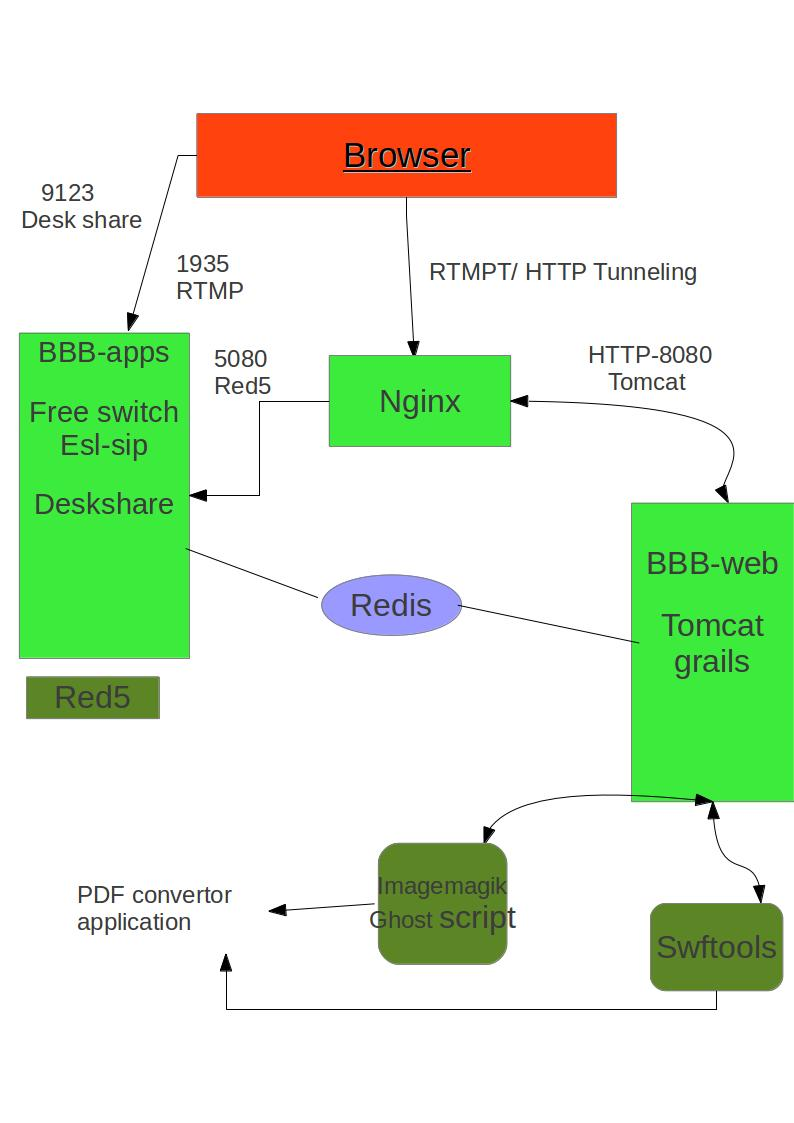
\includegraphics[height=90mm,width=90mm,angle=360]{./images/bbb-arch.jpg}
\end{small}
\end{frame}


%\section{Prerequisites}
\subsection*{bbb-apps}
\begin{frame}
\frametitle{Client communication with bbb-apps }
\begin{small}

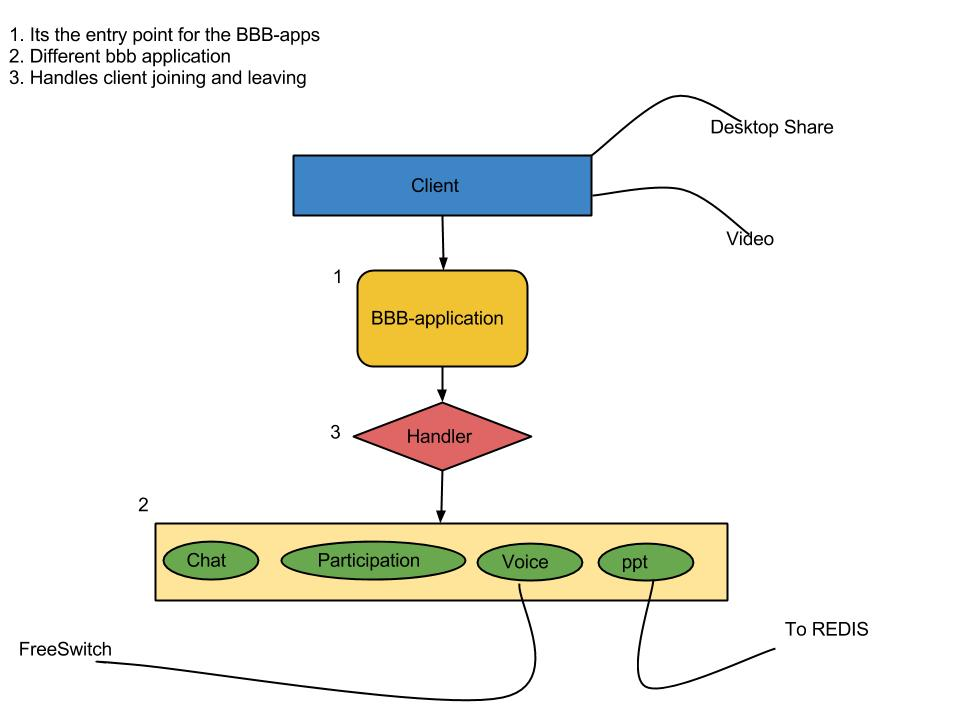
\includegraphics[height=70mm,width=90mm,angle=360]{./images/bbb-apps.jpg}
\end{small}
\end{frame}


\subsection*{ppt-upload}
\begin{frame}
\frametitle{Uploading presentation}

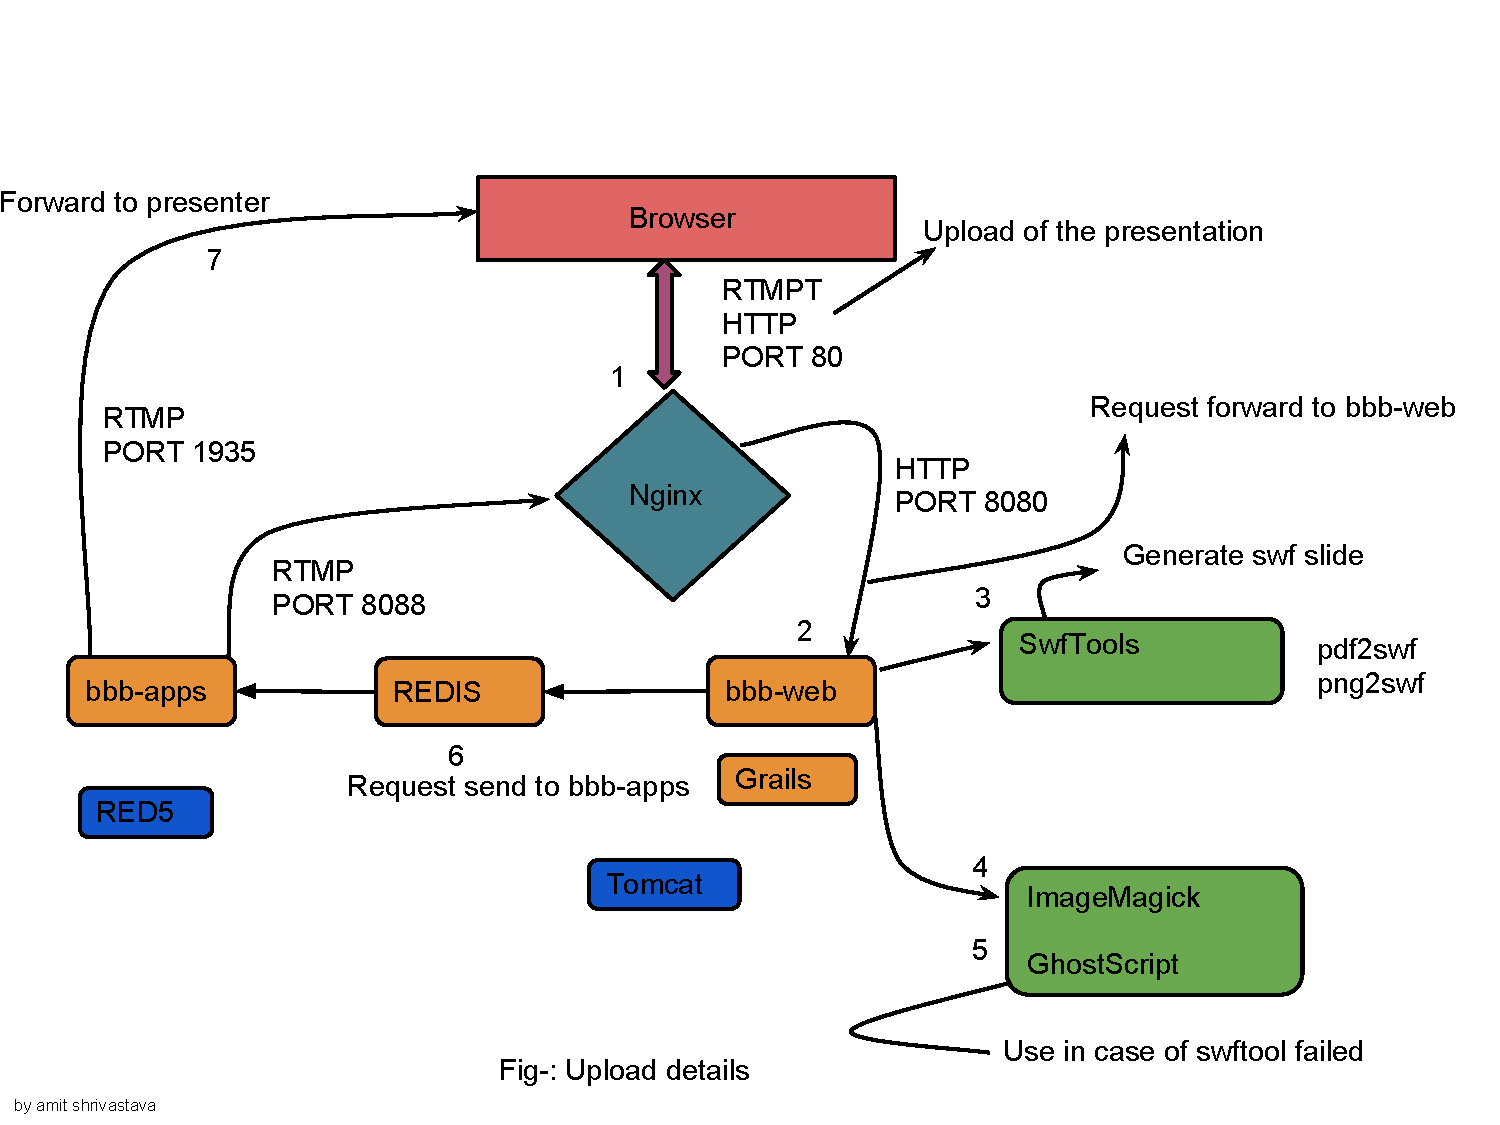
\includegraphics[height=70mm,width=90mm,angle=360]{./images/bbb-upload.pdf}
\end{frame}
%%%%%%%%%%%%%%%%%%%%%%%%%%%%%% 3

\section{Tools}
\subsection*{List}
\begin{frame}
\frametitle{List of Components }
\begin{small}

\begin{itemize}
        \item{Ubuntu 10.04}
	\item{Ghostscript}
        \item{ActiveMQ}
        \item{RED5}
        \item{Tomcat6}
	\item{Freeswitch}
	\item{PopcornJS}
	\item{FlexSDK}	
	\item{Grails}
	\item{Image Magick}
	\item{Nginx}
	\item{swfTool}
	\item{REDIS}
 \end{itemize}
	\end{small}
\end{frame}





%%%%%%%%%%%%%%%%%%%%%%%%%%% 4
\section{Source code}
\subsection*{Directories}
\begin{frame}
\frametitle{List of Directories}
{There are total 13 directories with different files}
\begin{small}
\begin{enumerate}

	\item{bbb-api-demo}
	\item{bbb-common-message}
	\item{bbb-lti}
	\item{bbb-video}
	\item{bbb-voice-conference}
	\item{bbb-voice}
	\item{bigbluebutton-apps}
	\item{bigbluebutton-client}
	\item{bigbluebutton-config}
	\item{bigbluebutton-web}
	\item{deskshare}
	\item{esl-client-bbb}
	\item record-and-playback 

\end{enumerate}
\end{small}
\end{frame}



\subsection*{Mindmap}
\begin{frame}
\frametitle{Tree structure of Directories}
{Full grown tree}


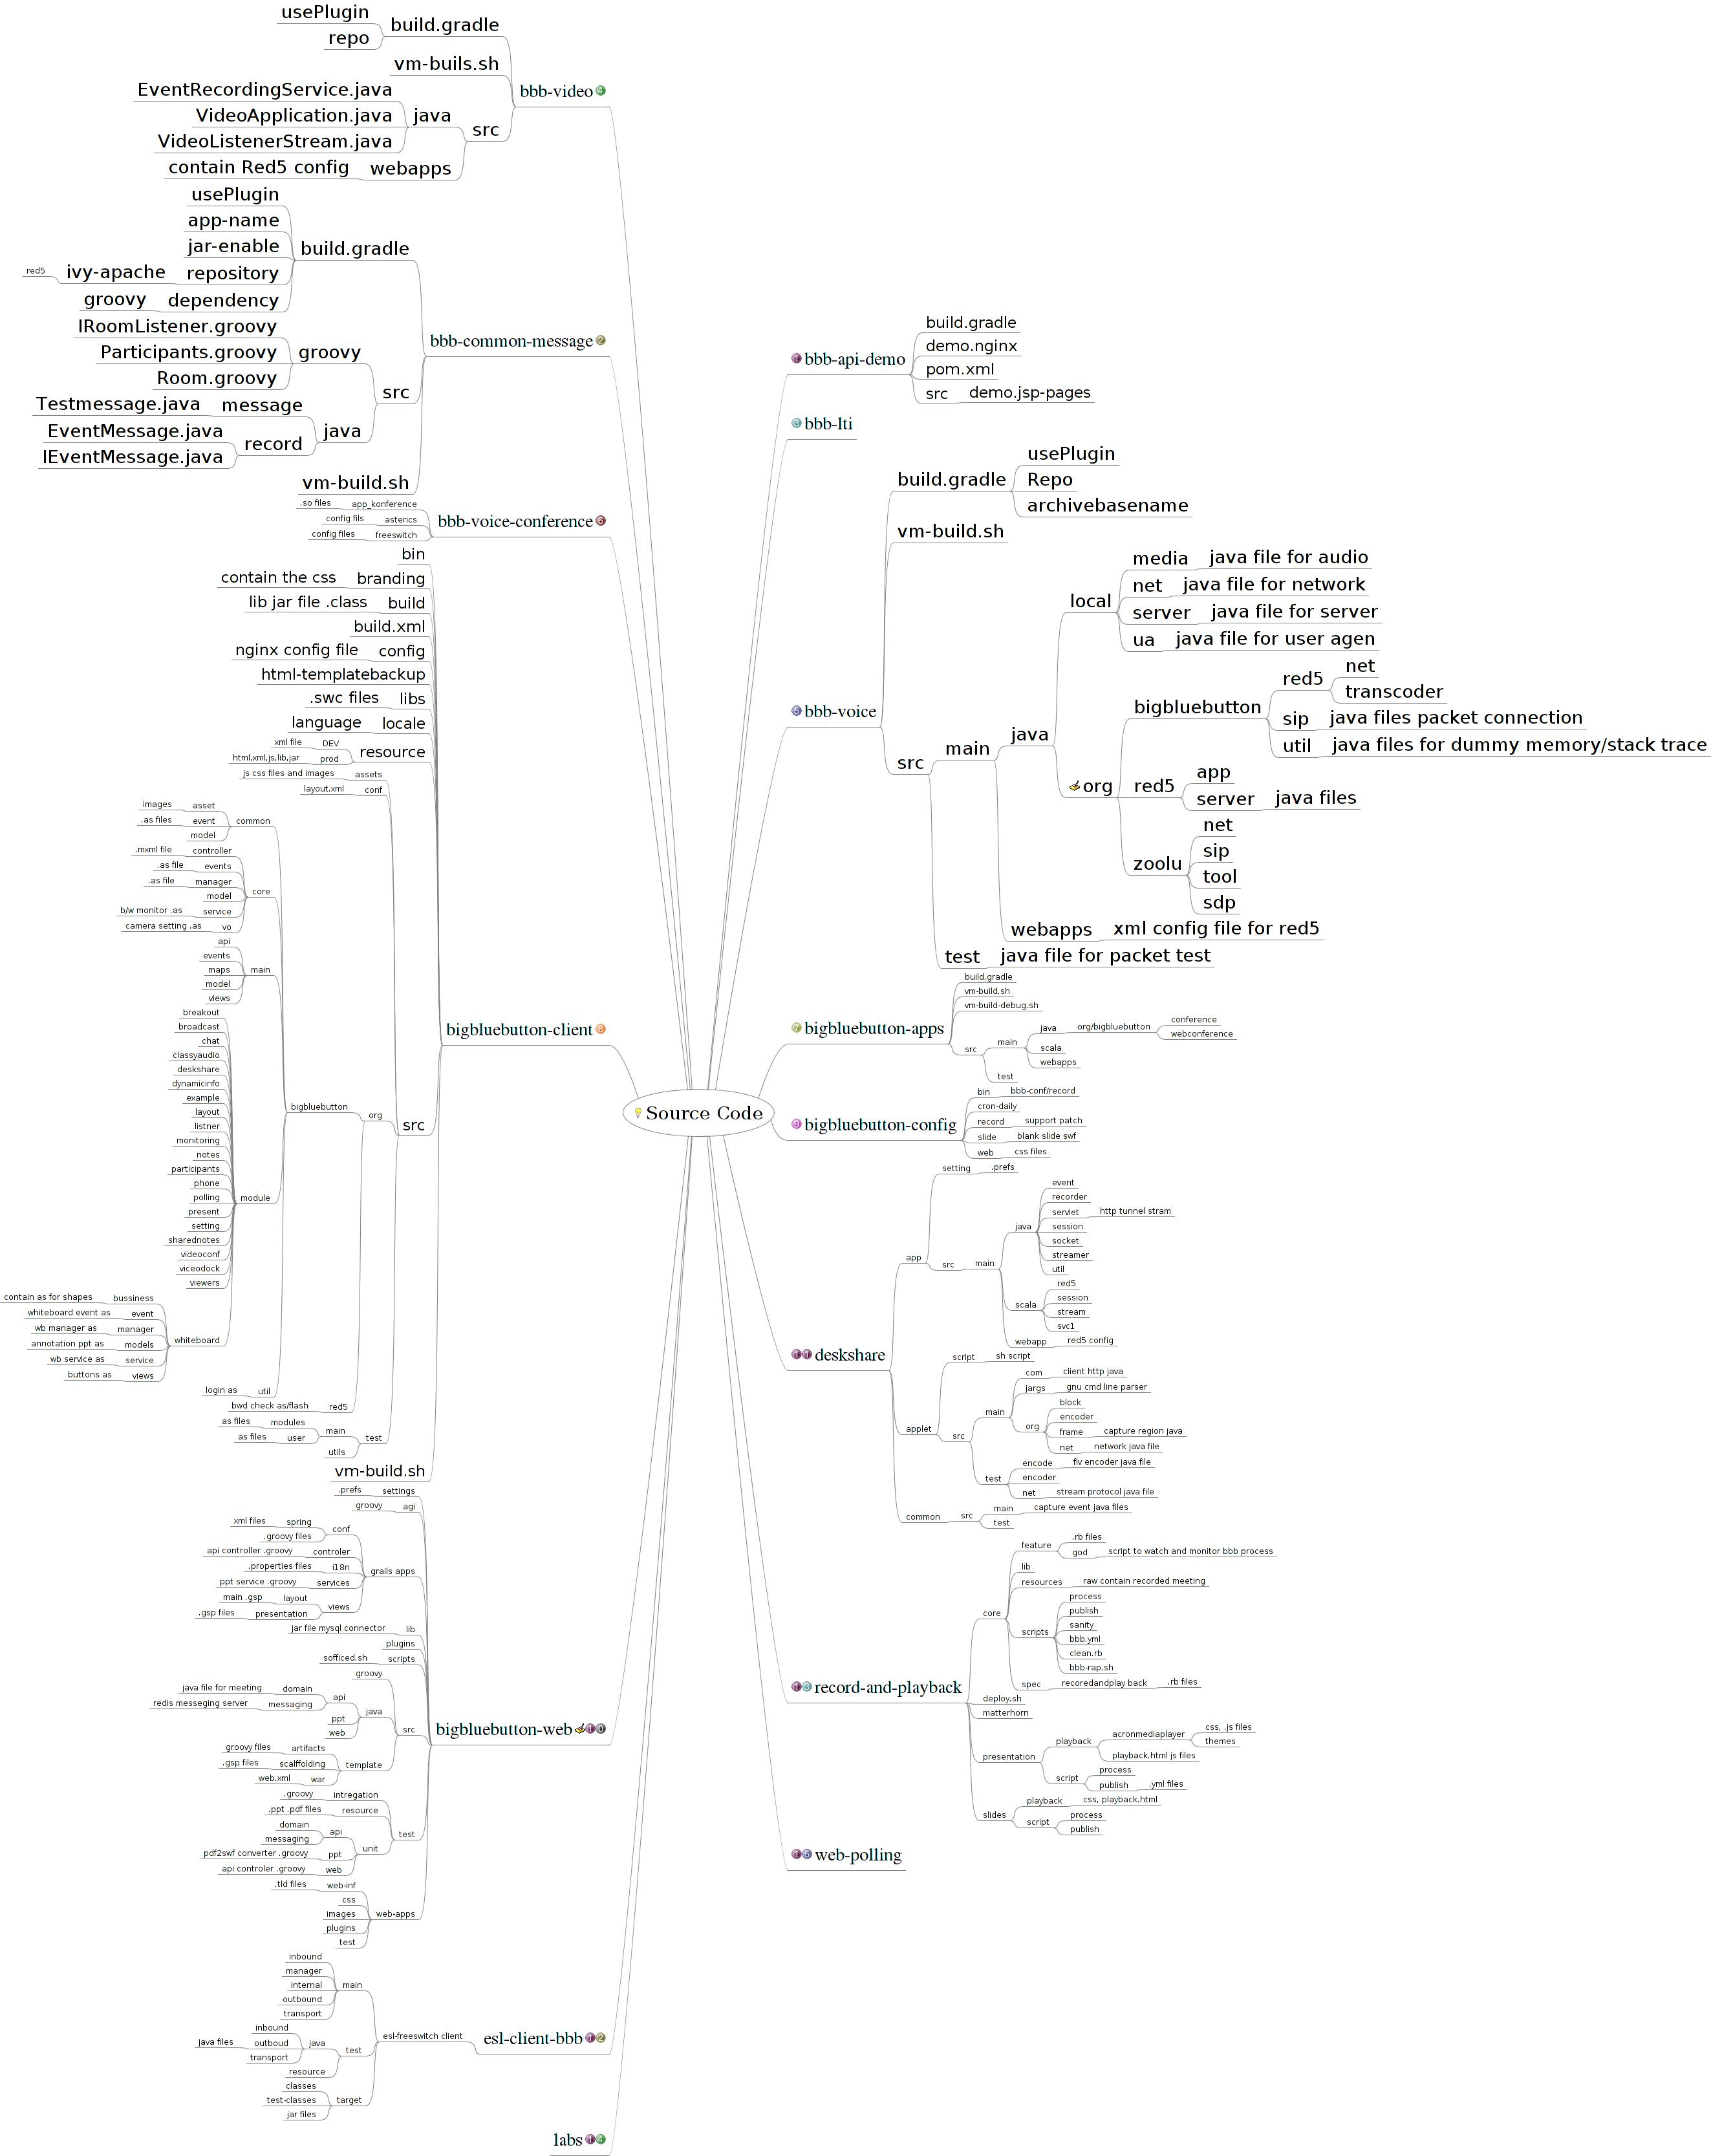
\includegraphics[height=70mm,width=90mm,angle=360]{./images/SourceCode.jpeg}
\end{frame}

\subsection*{Mindmap}
\begin{frame}
\frametitle{Tree structure of Directories}
{Close tree}

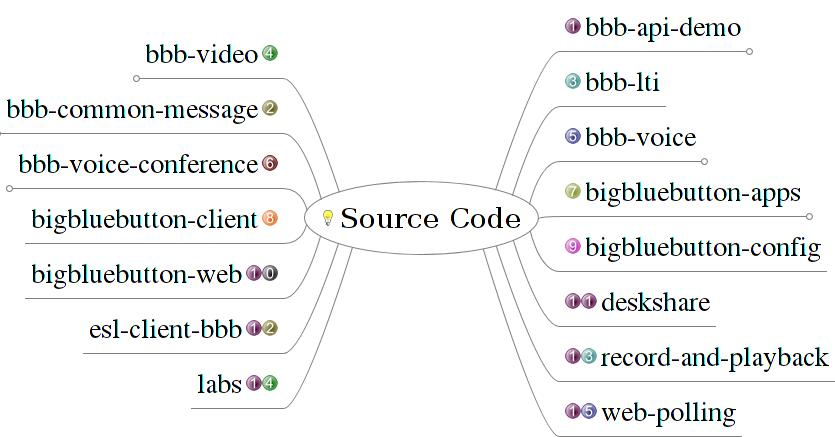
\includegraphics[height=70mm,width=90mm]{./images/SourceCodeintro.jpeg}
\end{frame}



\subsection*{Mindmap}
\begin{frame}
\frametitle{Tree structure of Directories}
{bbb-api expand tree }

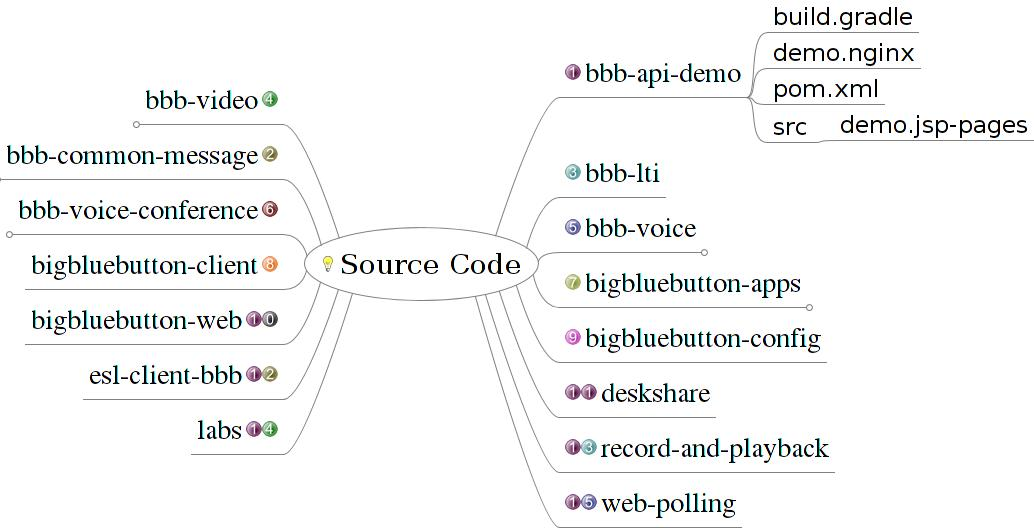
\includegraphics[height=70mm,width=90mm]{./images/SourceCode1.jpeg}
\end{frame}



\subsection*{Mindmap}
\begin{frame}
\frametitle{Tree structure of Directories}
{bbb-common-message expand tree }

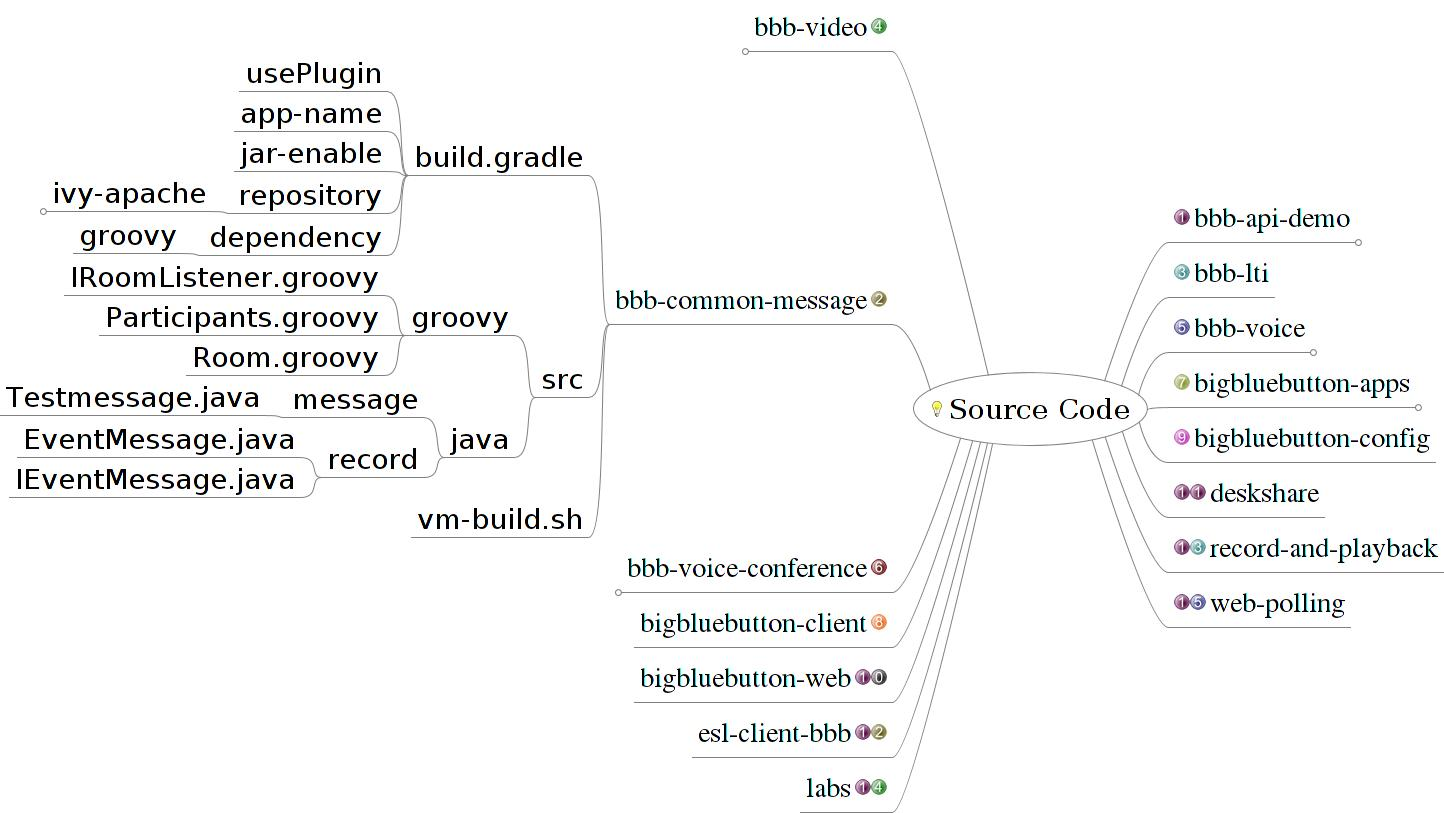
\includegraphics[height=70mm,width=90mm]{./images/SourceCode2.jpeg}
\end{frame}



\subsection*{Mindmap}
\begin{frame}
\frametitle{Tree structure of Directories}
{bbb-common-message expand tree }

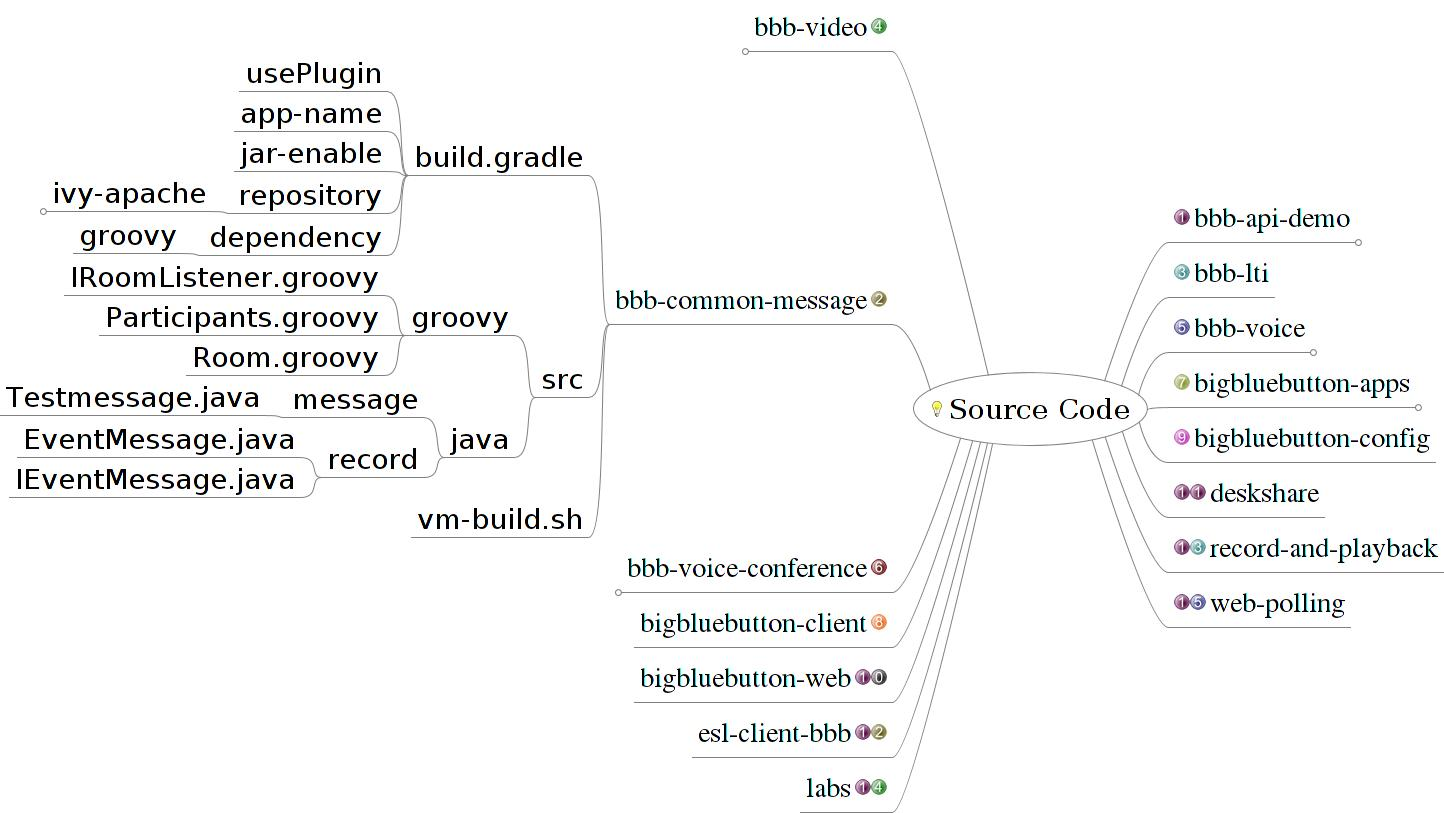
\includegraphics[height=70mm,width=90mm]{./images/SourceCode2.jpeg}
\end{frame}


\subsection*{Mindmap}
\begin{frame}
\frametitle{Tree structure of Directories}
{bbb-video expand tree}

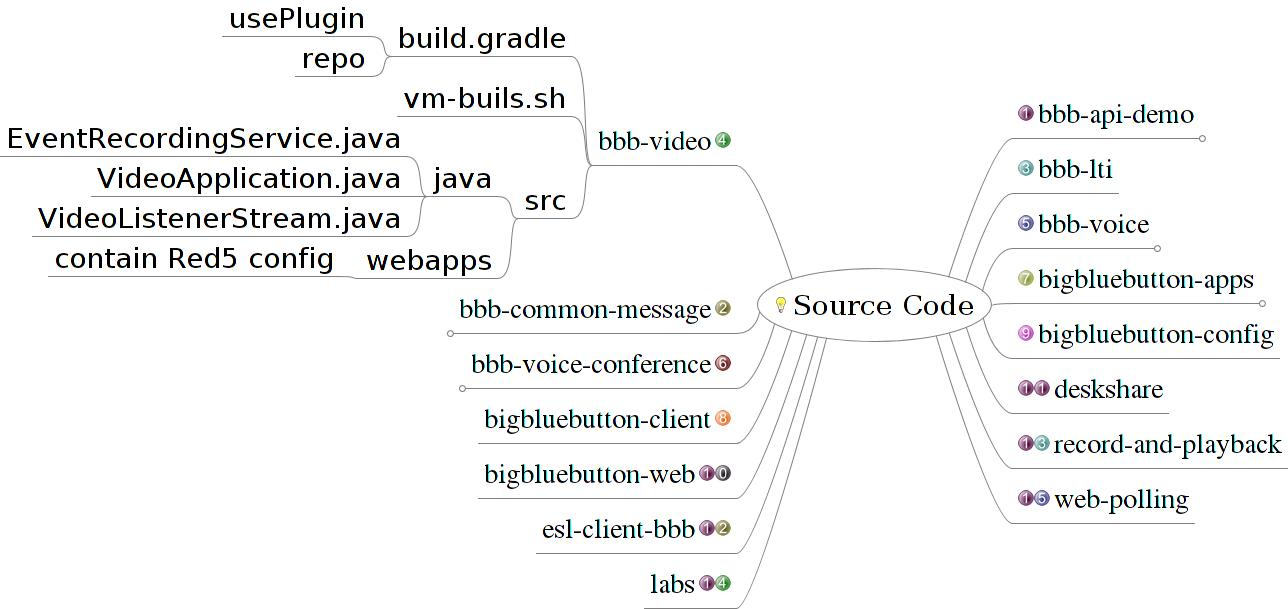
\includegraphics[height=70mm,width=90mm]{./images/SourceCode4.jpeg}
\end{frame}



\subsection*{Mindmap}
\begin{frame}
\frametitle{Tree structure of Directories}
{bbb-voice expand tree}

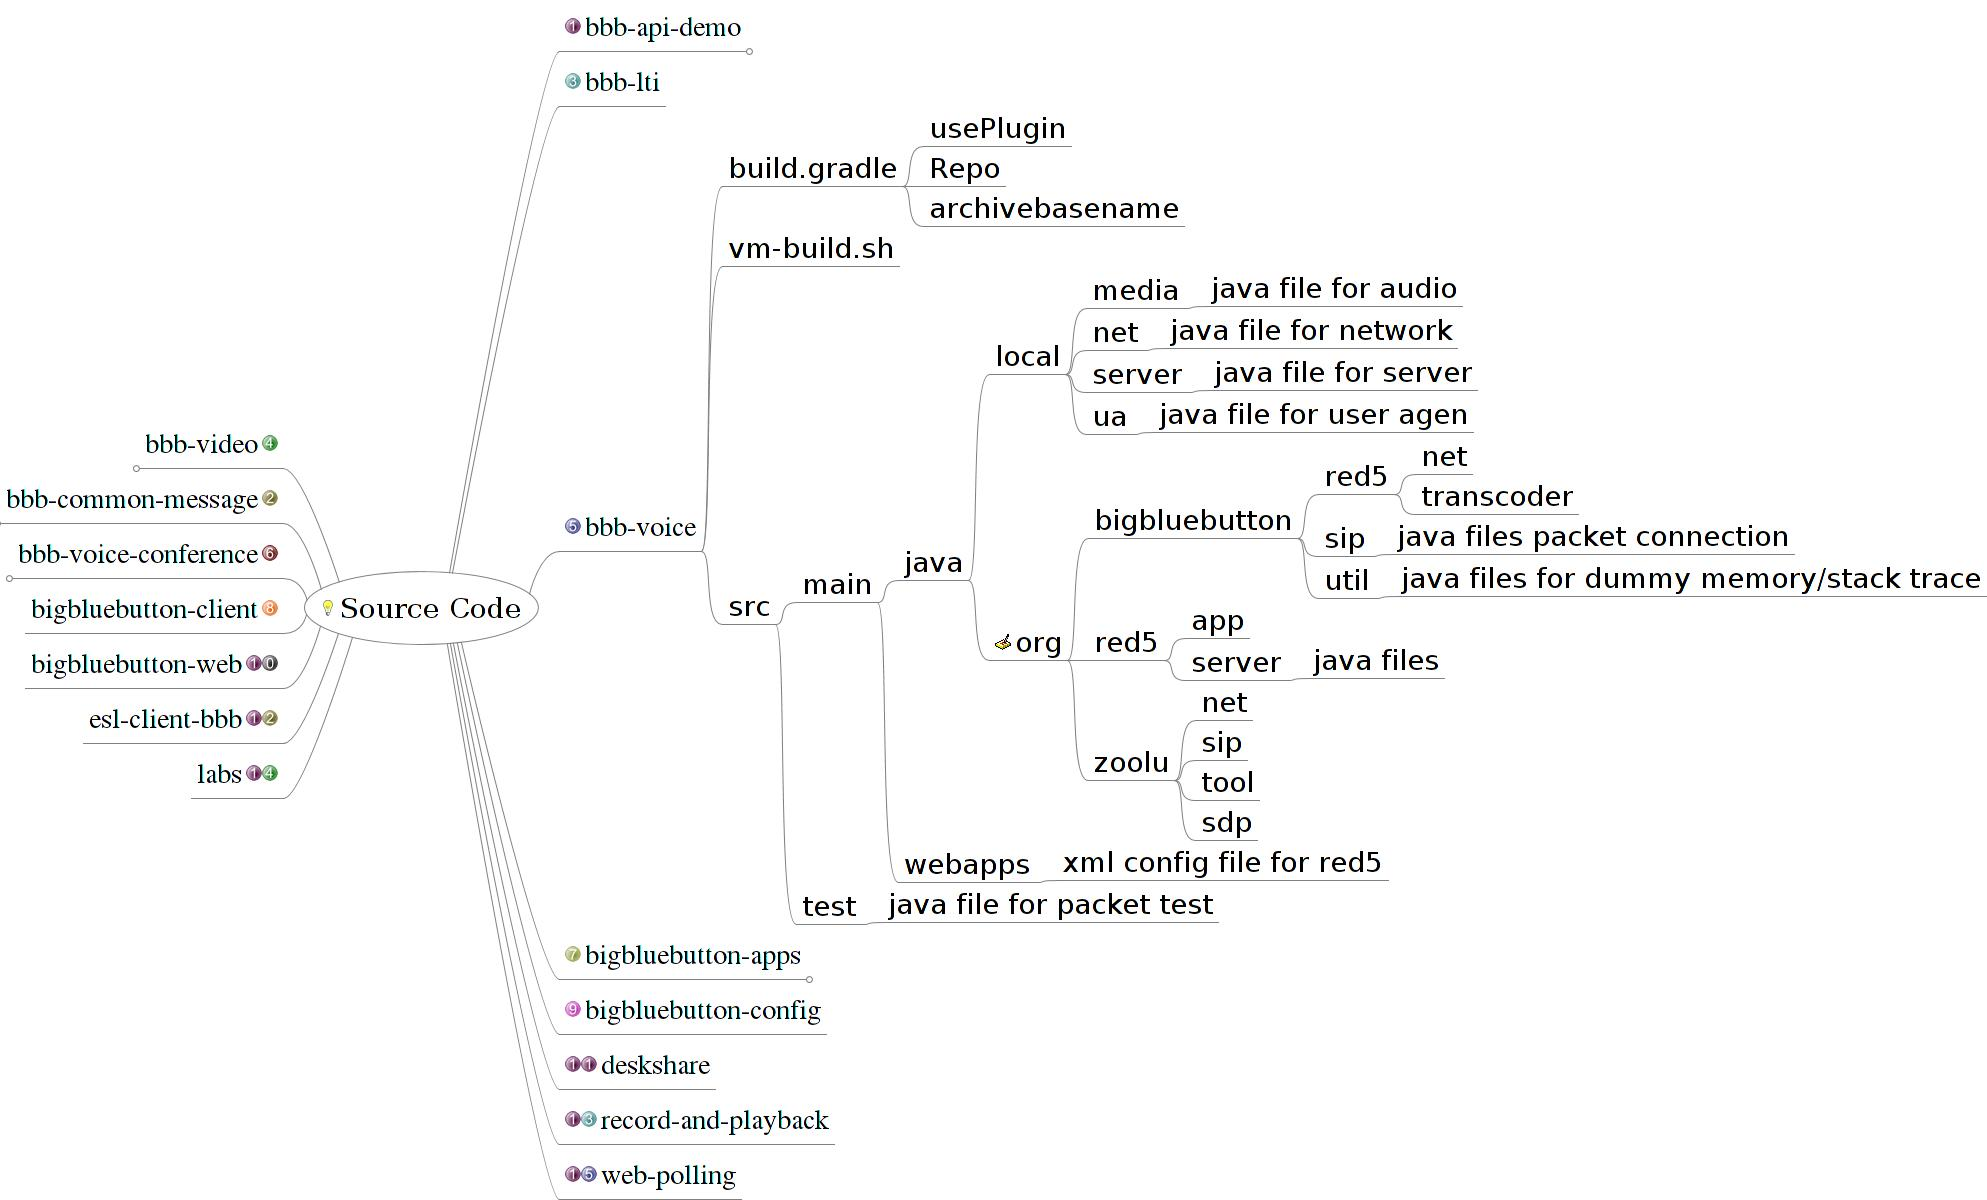
\includegraphics[height=70mm,width=90mm]{./images/SourceCode5.jpeg}
\end{frame}


\subsection*{Mindmap}
\begin{frame}
\frametitle{Tree structure of Directories}
{bbb-voice-conference expand tree}
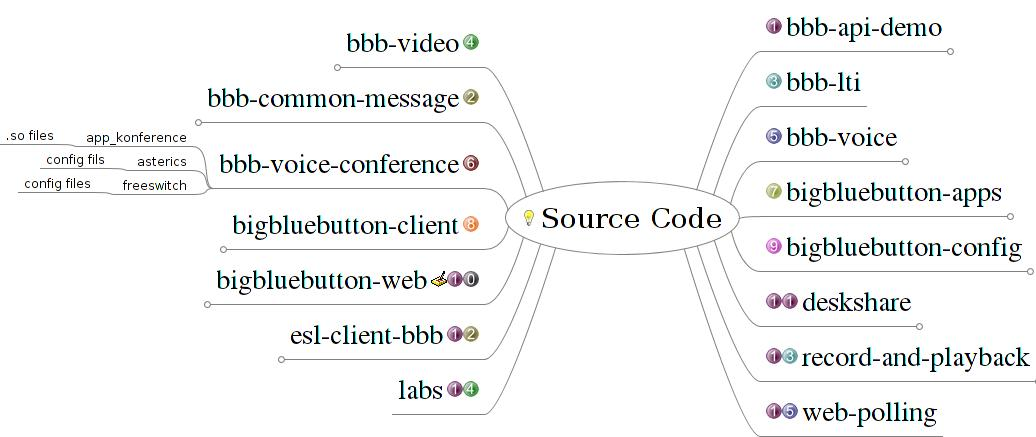
\includegraphics[height=70mm,width=90mm]{./images/SourceCode6.jpeg}
\end{frame}

\subsection*{Mindmap}
\begin{frame}
\frametitle{Tree structure of Directories}
{bbb-apps expand tree}
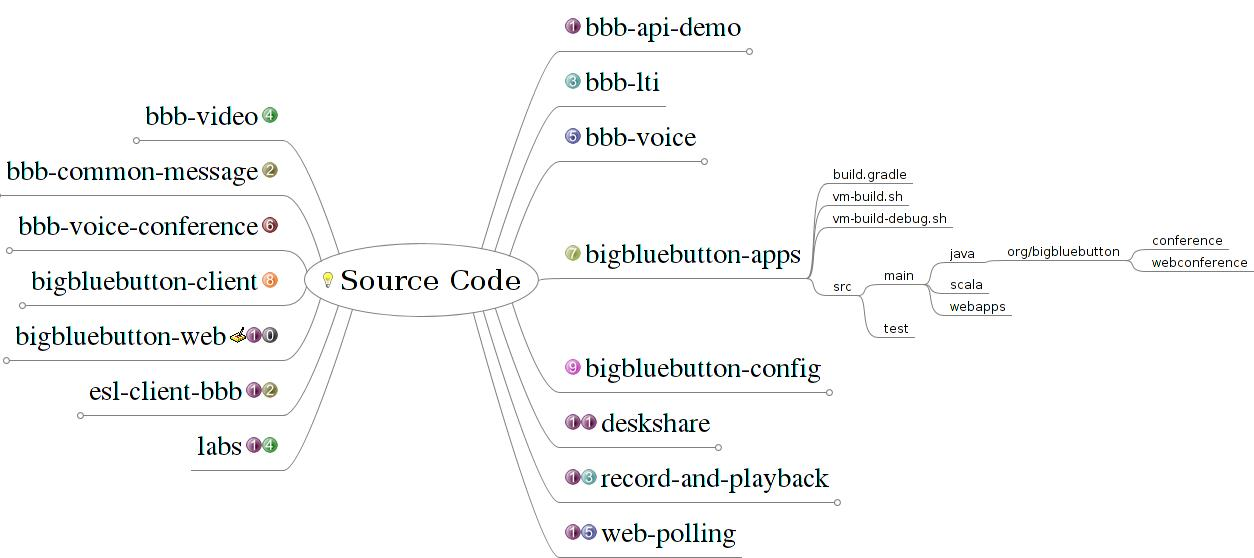
\includegraphics[height=70mm,width=90mm]{./images/SourceCode7.jpeg}
\end{frame}




\subsection*{Mindmap}
\begin{frame}
\frametitle{Tree structure of Directories}
{bbb-client expand tree}
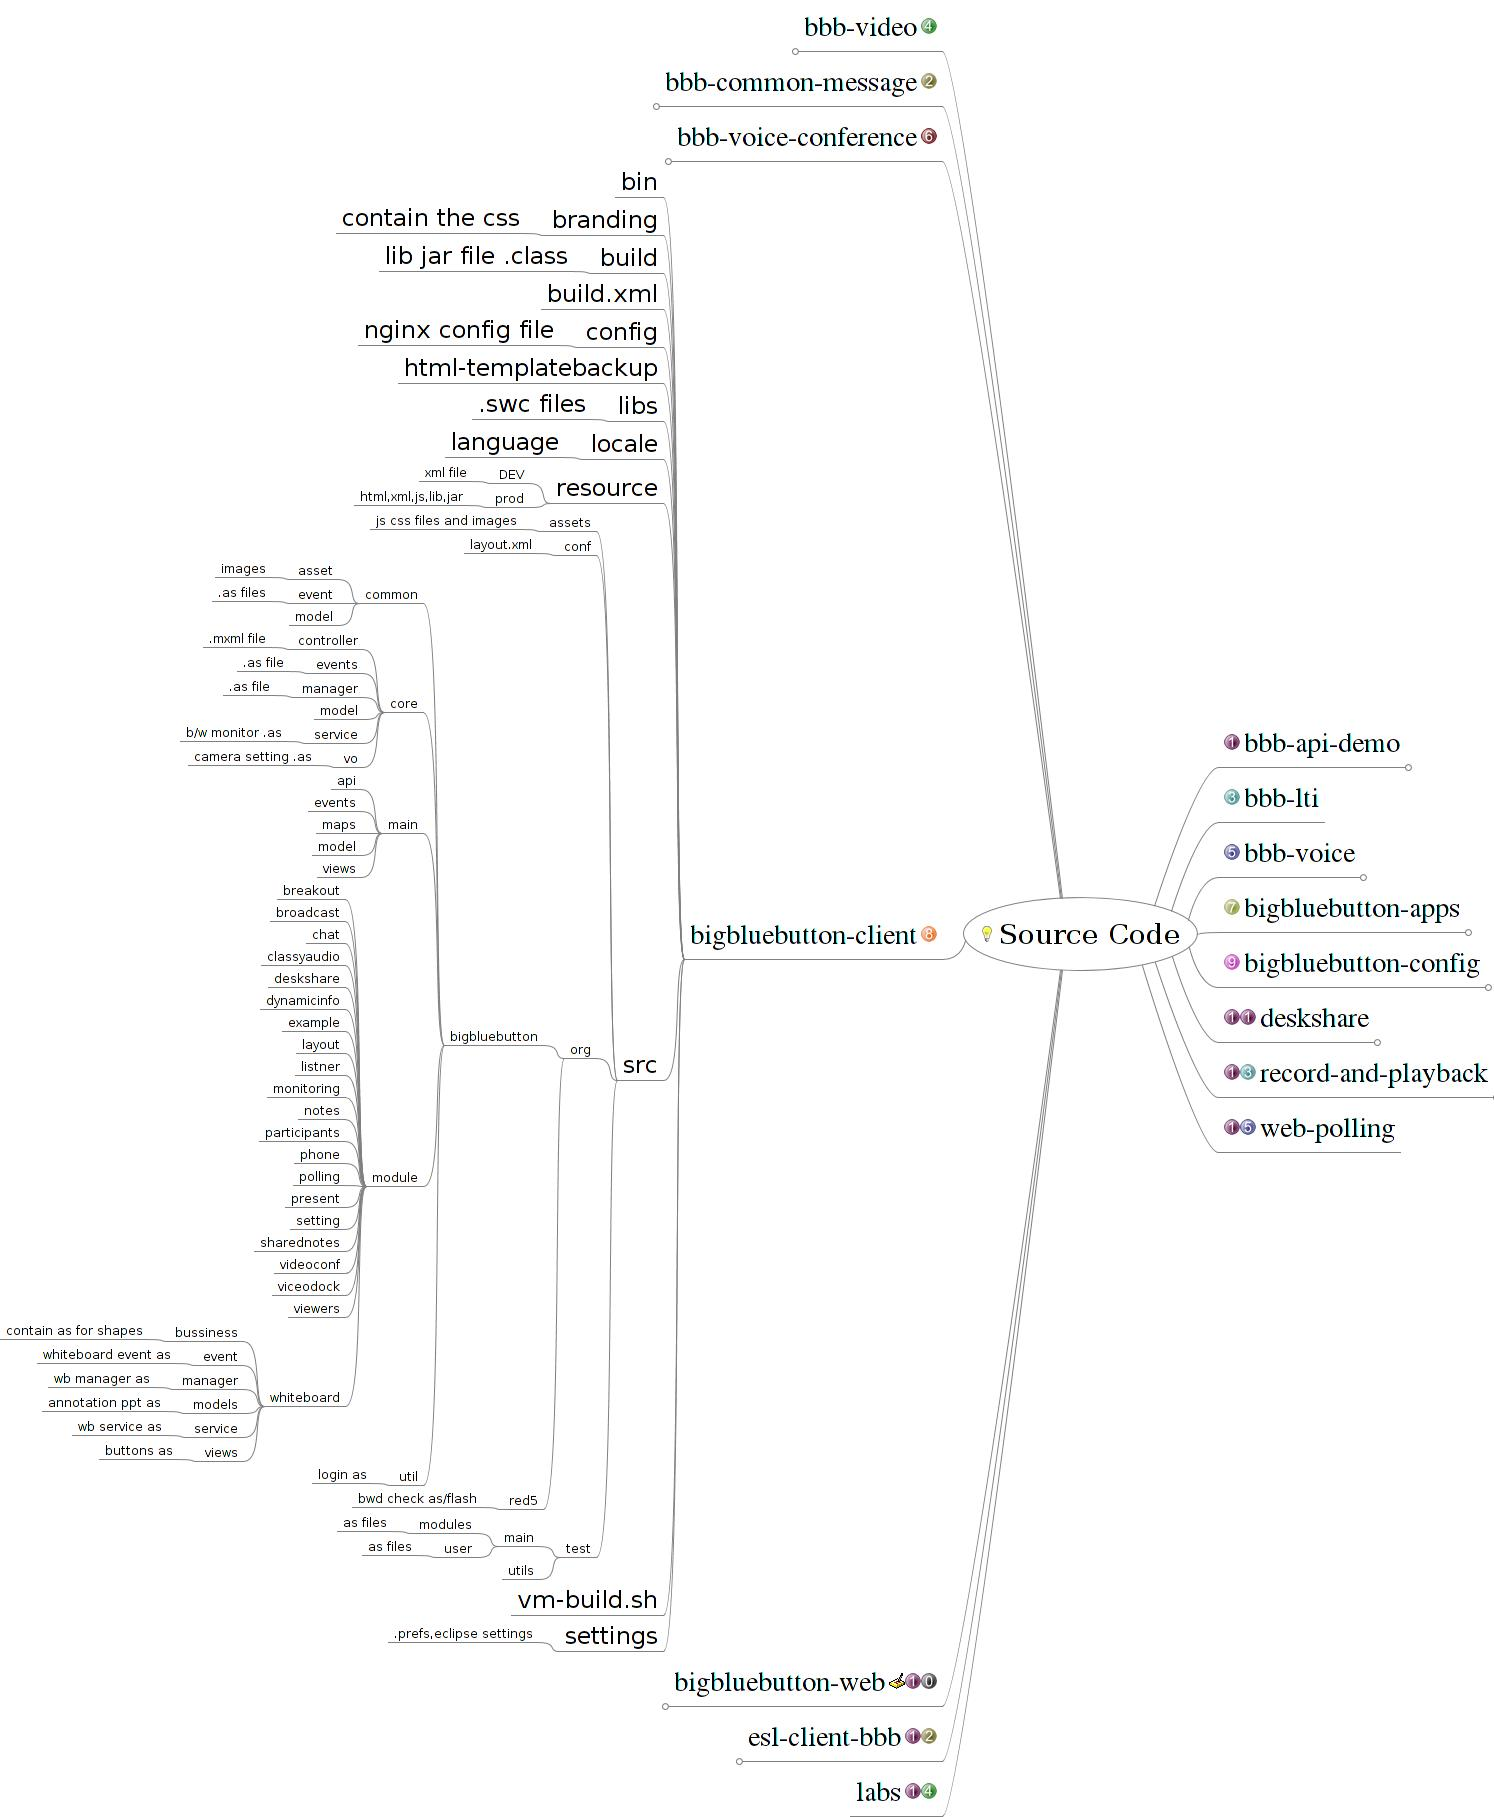
\includegraphics[height=70mm,width=90mm]{./images/SourceCode8.jpeg}
\end{frame}


\subsection*{Mindmap}
\begin{frame}
\frametitle{Tree structure of Directories}
{bbb-config expand tree}
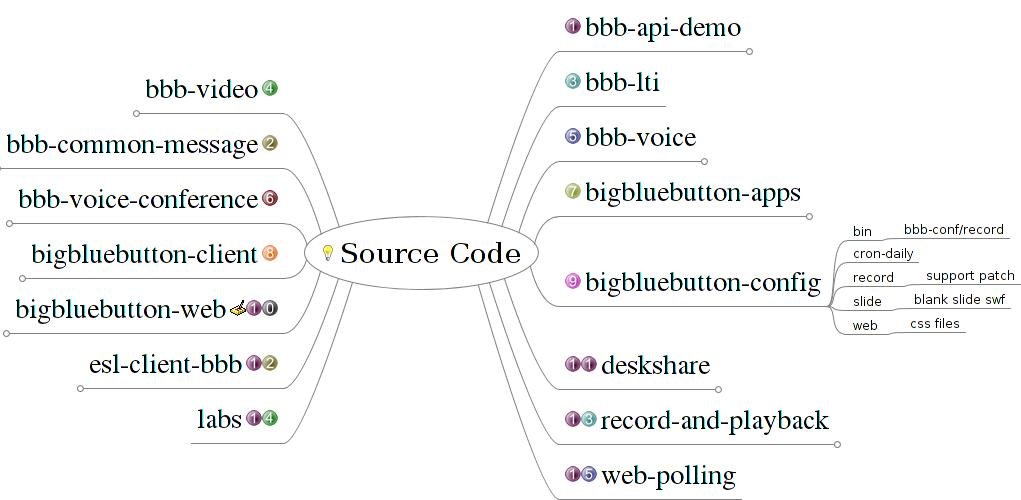
\includegraphics[height=70mm,width=90mm]{./images/SourceCode9.jpeg}
\end{frame}


\subsection*{Mindmap}
\begin{frame}
\frametitle{Tree structure of Directories}
{bbb-web expand tree}
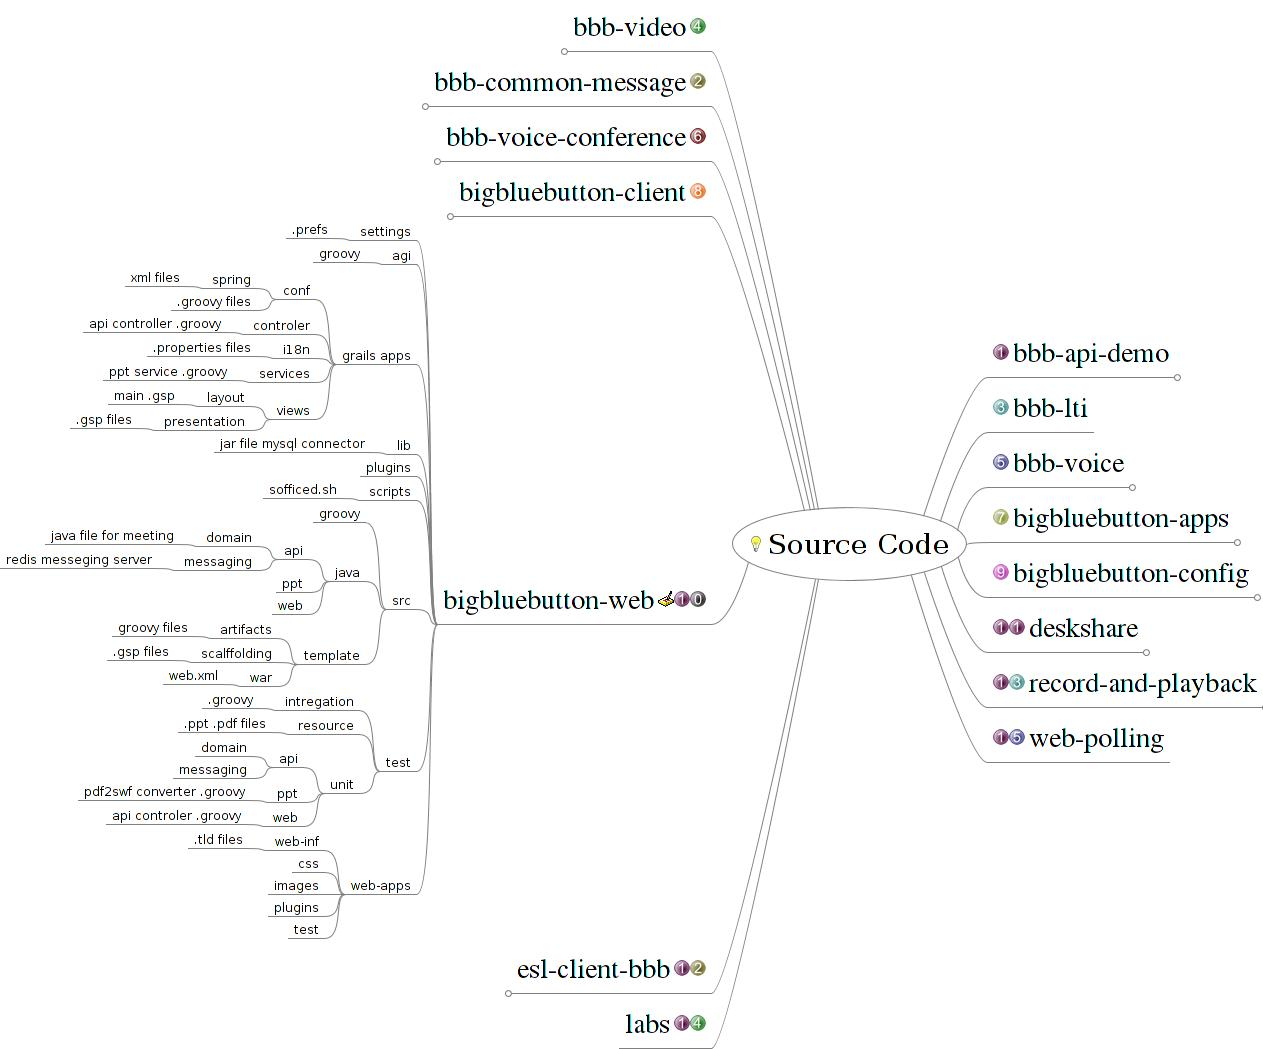
\includegraphics[height=70mm,width=90mm]{./images/SourceCode10.jpeg}
\end{frame}


\subsection*{Mindmap}
\begin{frame}
\frametitle{Tree structure of Directories}
{bbb-deskshare expand tree}
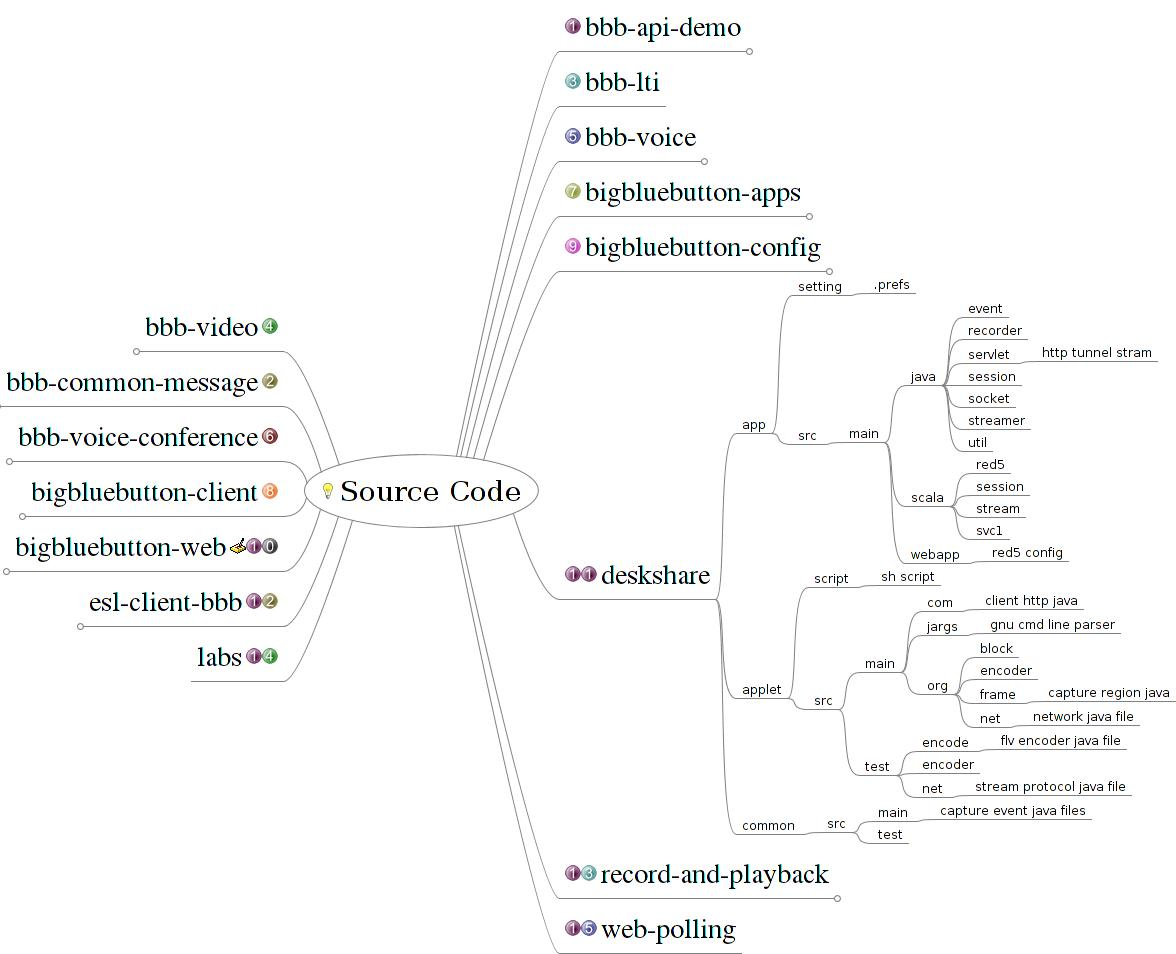
\includegraphics[height=70mm,width=90mm]{./images/SourceCode11.jpeg}
\end{frame}


\subsection*{Mindmap}
\begin{frame}
\frametitle{Tree structure of Directories}
{bbb-esl-client expand tree}
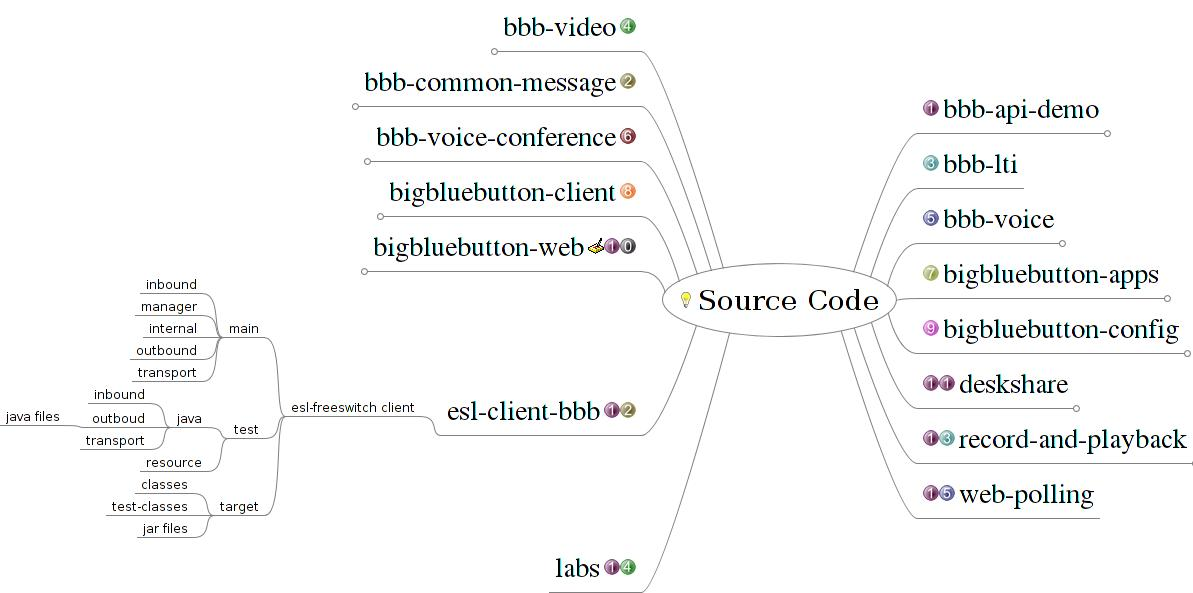
\includegraphics[height=70mm,width=90mm]{./images/SourceCode12.jpeg}
\end{frame}


\subsection*{Mindmap}
\begin{frame}
\frametitle{Tree structure of Directories}
{bbb-record and playback expand tree}
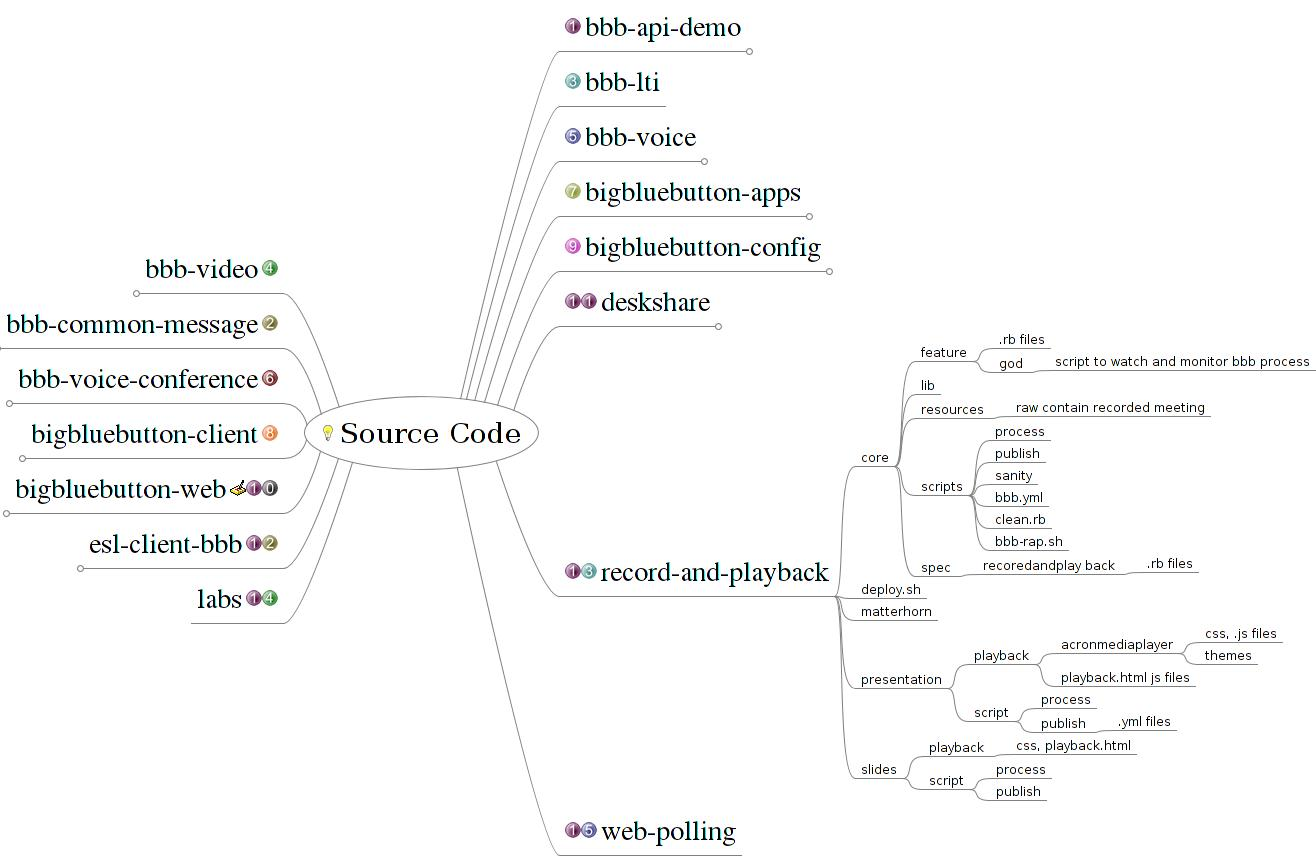
\includegraphics[height=70mm,width=90mm]{./images/SourceCode13.jpeg}
\end{frame}


\subsection*{Mindmap}
\begin{frame}
\frametitle{Tree structure of Directories}
{bbb-apps expand tree}
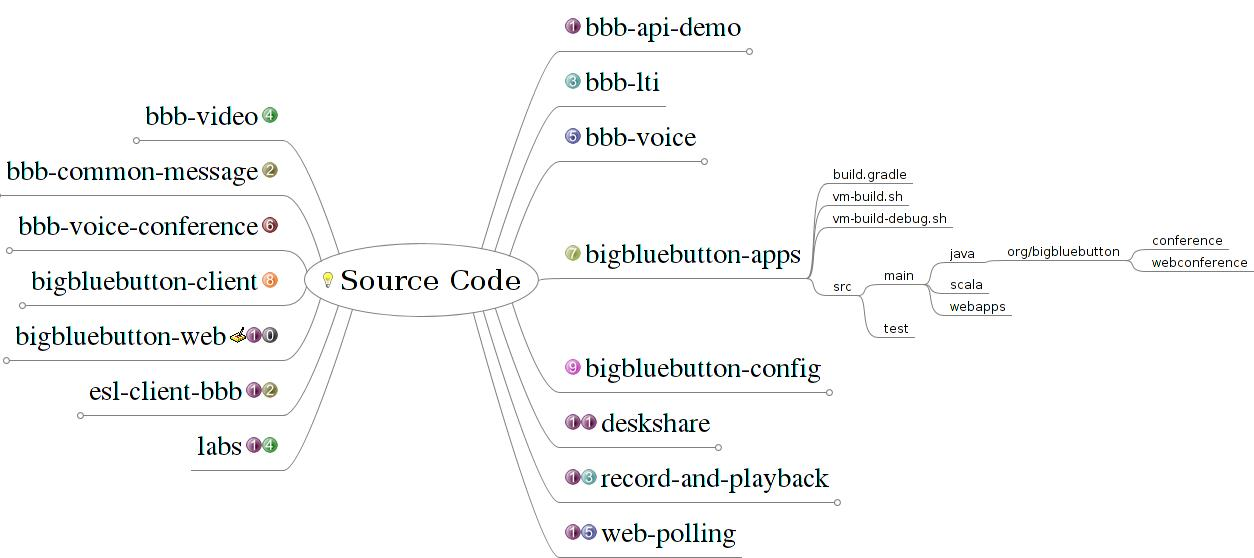
\includegraphics[height=70mm,width=90mm]{./images/SourceCode7.jpeg}
\end{frame}
%%%%%%%%%%%%%%%%%%%%%%%%%%% 6 





%%%%%%%%%%%%%%%%%%%5555
%\begin{frame}
%\addtocounter{framenumber}{-1}
%%	\frametitle{Bibliography:}
%\tiny
%\begin{thebibliography}{50}
%\addtolength{\leftmargin}{0.2in} % sets up alignment with the following line.
%\setlength{\itemindent}{-0.2in}
%
%
%\bibitem{Doy} K. Zhou, J.C. Doyle, K. Glover, et al., Robust and optimal control, vol. 40, Prentice
%Hall Upper Saddle River, NJ, 1996.
%
%\bibitem{Ander} 
%B.D.O. Anderson and S. Vongpanitlerd, Network analysis and synthesis: a modern
%systems theory approach, Courier Dover Publications, 2006.
%
%\bibitem{Marin}T. Martinez-Marin, “State-space formulation for circuit analysis,” Education, IEEE
%Transactions on, vol. 53, no. 3, pp. 497–503, 2010.
%
%\bibitem{statespace}
%D.C. Karamousantas, G.E. Chatzarakis, G.N. Korres, and P.J. Katsikas, “Obtaining
%state equations for planar nondegenerate linear electric circuits using mesh analysis
%with virtual voltage sources,” International Journal of Electrical Engineering Educa-
%tion, vol. 45, no. 3, pp. 239–250, 2008.
%
%\bibitem{StateNat}
%S. Natarajan, “A systematic method for obtaining state equations using mna,” in
%Circuits, Devices and Systems, IEE Proceedings G. IET, 1991, vol. 138, pp. 341–346.
%
%\bibitem{ss}
%D.L. Skaar, “Using the superposition method to formulate the state variable matrix
%for linear networks,” Education, IEEE Transactions on, vol. 44, no. 4, pp. 311–314,
%2001.
%
%
%
%
%\end{thebibliography}
%\end{frame}
\addtocounter{framenumber}{-1}
\section*{}
\subsection*{}
\begin{frame}
	\begin{block}{\Large \bf {Thank You}}
	\end{block}
\end{frame}

\end{document}

%%%%%%%%%%%%%%%%%%%%%%%%%%%%%%%%%%%%%%%%%%%%%%%%%%%%%%%%%%%%%%%%%%%%%%%%%%%%%%%%%%%%%%%%%%%%%%%%%%%%%%%%%%%%%%%%


